\documentclass[12pt,a4paper]{article}
\usepackage[T2A]{fontenc}
\usepackage[utf8]{inputenc}
\usepackage[russian]{babel}
\usepackage{amsmath}
\usepackage{amssymb}
\usepackage{graphicx}
\usepackage{floatrow}
\usepackage{booktabs}
%\usepackage{wrapfig}
\usepackage{lipsum}
%\usepackage{subcaption}
\usepackage{fancyhdr}
\usepackage{mathrsfs}

%multi-column
%\multicolumn{number cols}{align}{text} % align: l,c,r

%multi-row
\usepackage{multirow}

\newcommand{\figref}[1]{(См. рис. \ref{#1})}
\newcommand{\secref}[1]{(См. раздел. \ref{#1})}

\newcommand{\e}[1]{\text{$\cdot10^{#1}$}}

\pagestyle{fancy}
\fancyhead{}
\fancyhead[L]{Работа 2.3.1}
\fancyhead[R]{}
\fancyfoot[C]{\thepage}

\renewcommand{\cot}{\text{ctg}}

\author{\normalsize Выполнил: Дедков Денис, группа Б01-109 \\
	\normalsize 19.11.2022}
\date{}

\usepackage{float}
\restylefloat{table}
\title{
	\large Отчет о выполнении лабораторной работы 3.2.2 \\
	\Large Резонанс напряжений в последовательном контуре \\ 
	
}

\begin{document}
\maketitle
\subsection*{Цель работы} Исследование резонанса напряжений в последовательном
колебательном контуре с изменяемой ёмкостью, получение амплитудночастотных и фазово-частотных характеристик, определение основных параметров контура.
\subsection*{Оборудование и приборы} Генератор сигналов, источник напряжения,
нагрузкой которого является последовательный колебательный контур с
переменной ёмкостью, двухканальный осциллограф, цифровые вольтметры.

\subsection*{Введение}

В данной работе изучаются резонансные явления в последовательном колебательном контуре (резонанс напряжений). Схема экспериментального стенда показана на рис. \ref{fig:scheme}. Синусоидальный сигнал от генератора поступает на вход управляемого напряжением источника напряжения, собранного на операционном усилителе.

В колебательный контур установки добавлен постоянный резистор $R$, снижающий его
добротность. Это сделано для упрощения процедур получения и обработки резонансных кривых. Таким образом, суммарное активное сопротивление контура принимается равным

$$R_{\Sigma} = R + R_L + R_S$$

Добротность контуров тем не менее остаётся достаточно высокой, чтобы
можно было пользоваться классическими формулами:

$$\mathcal{Q} = \frac{\rho}{R_{\Sigma}} = \frac{\omega_0 L}{R_{\Sigma}} 
= \frac{1}{\omega_0 C R_{\Sigma}} \gg 1$$

При резонансе, когда для высокодобротного контура можно положить $\omega = \omega_0$, выражения для модулей комплексных амплитуд тока и напряжения на ёмкости и их фаз принимают простой вид:

$$I(\omega_0) = \frac{\mathscr{E}}{R_{\Sigma}},\;\; U_C(\omega_0) = \mathcal{Q} \mathscr{E}, \;\; U_L(\omega_0) = \mathcal{Q} \mathscr{E}.$$

\begin{figure}[H]
	\centering
	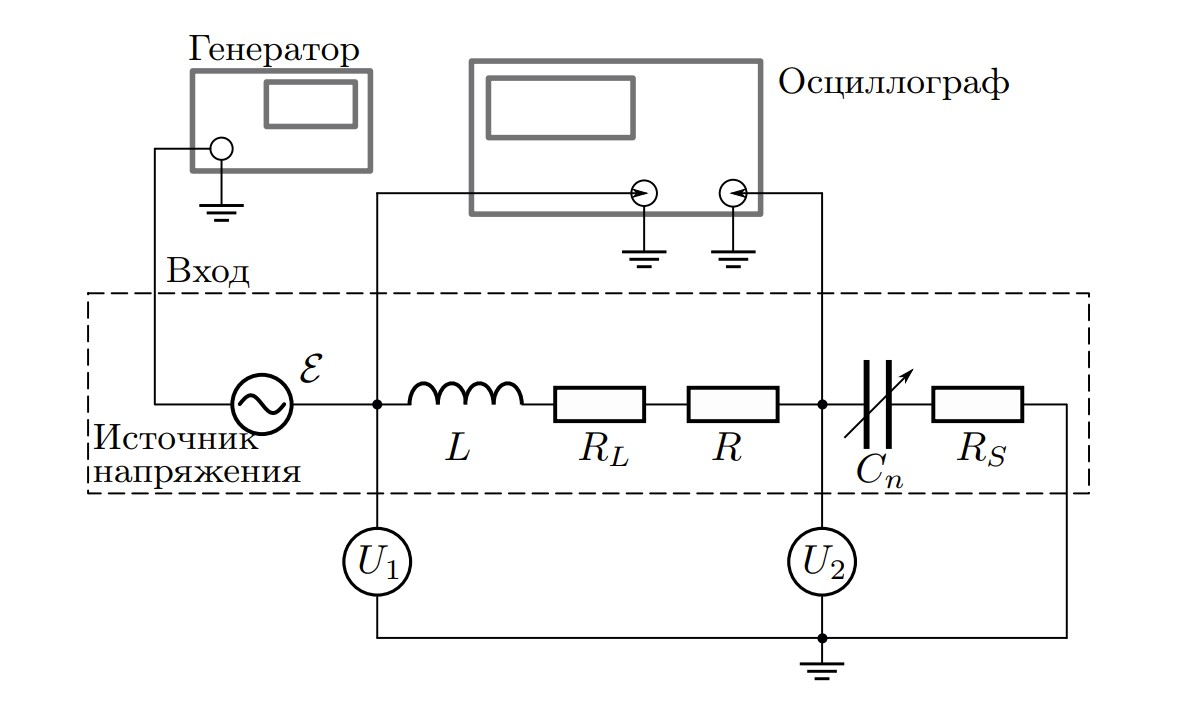
\includegraphics[scale = 0.4]{res/scheme.jpg}
	\caption{Схема экспериментального стенда}
	\label{fig:scheme}
\end{figure}

	
\subsection*{Ход работы}

Для контуров с различными ёмкостями $C_n$, меняя их с помощью переключателя на блоке, измерим резонансные частоты $f_0$ и напряжения $U_C$ при установленном в напряжении $\mathscr{E}$ на выходе генератора. Для каждого значения $C_n$ по данным эксперимента проведем расчёт параметров стенда (см. таблицу \ref{tab:params}).

Рассчитаем средние значения $L$ и $R_L$ и их случайные погрешности для использования в дальнейшем (см. таблицу \ref{tab:RL}).

\begin{table}[H]
	\footnotesize
	\input{gen/setup.tex}
	\caption{Параметры контура}
	\label{tab:params}
\end{table}

\begin{table}[H]
	\footnotesize
	\input{gen/setup-mean.tex}
	\caption{Погрешности параметров}
	\label{tab:RL}
\end{table}

Построим графики амплитудно-частотные характеристик $U_C(f)$ для выбранных контуров (см. рис. \ref{fig:resonance}).

\begin{figure}[h]
	\centering
	\includegraphics[scale = 0.8]{gen/fig-resonance.pdf}
	\caption{Графики амплитудно-частотные характеристик}
	\label{fig:resonance}
\end{figure}

\clearpage

Для контуров с двумя разными ёмкостями измерим амплитудно-частотные $U_C(f)$ и  фазово-частотные $\varphi(f)$ характеристики (см. таблицу \ref{tab:norm}).


Построим на одном графике амплитудно-частотные характеристики в безразмерных координатах $x = \frac{f}{f_0}$, $y = \frac{U_C}{U_C(f_0)}$. По ширине резонансных кривых на уровне 0,707
определим добротности $\mathcal{Q}$ соответствующих контуров:

$$\mathcal{Q}\left(33.2 \text{ нФ}\right) = 22.6 \pm 0.5$$
$$\mathcal{Q}\left(68 \text{ нФ}\right) = 16.6 \pm 0.3$$

\begin{figure}[H]
	\centering
	\includegraphics[scale = 0.8]{gen/fig-resonance-norm.pdf}
	\caption{Графики амплитудно-частотные характеристик в нормированных координатах}
	\label{fig:norm}
\end{figure}


Построим на одном графике фазово-частотные характеристики в безразмерных координатах $x = \frac{f}{f_0}$, $y = \frac{\varphi}{\pi}$. По этим характеристикам определим добротности контуров по расстоянию между точками по оси $x$, в которых $y$ меняется от $1/4$ до $3/4$:

$$\mathcal{Q}\left(33.2 \text{ нФ}\right) = 20.7 \pm 0.4$$
$$\mathcal{Q}\left(68 \text{ нФ}\right) = 14.5 \pm 0.2$$


\begin{table}[H]
	\footnotesize
	\caption{Погрешности параметров}
	\input{gen/measure.tex}
	\label{tab:norm}
\end{table}



\begin{figure}[H]
	\centering
	\includegraphics[scale = 0.8]{gen/fig-phase.pdf}
	\caption{Пробная катушка и ее положение относительно магнита}
\end{figure}

\subsection*{Вывод}
В работе был исследован резонанс напряжений в последовательном колебательном контуре с изменяемой ёмкостью. Также получены амплитудно-частотные и фазово-частотные характеристики.

Несколькими методами была посчитана добротность контура. Результаты неплохо согласуются друг с другом.


\end{document}